\documentclass[border=3pt]{standalone}
\usepackage{times}
\usepackage{tikz}
\usetikzlibrary{positioning,arrows.meta,fit,backgrounds,calc}
\begin{document}
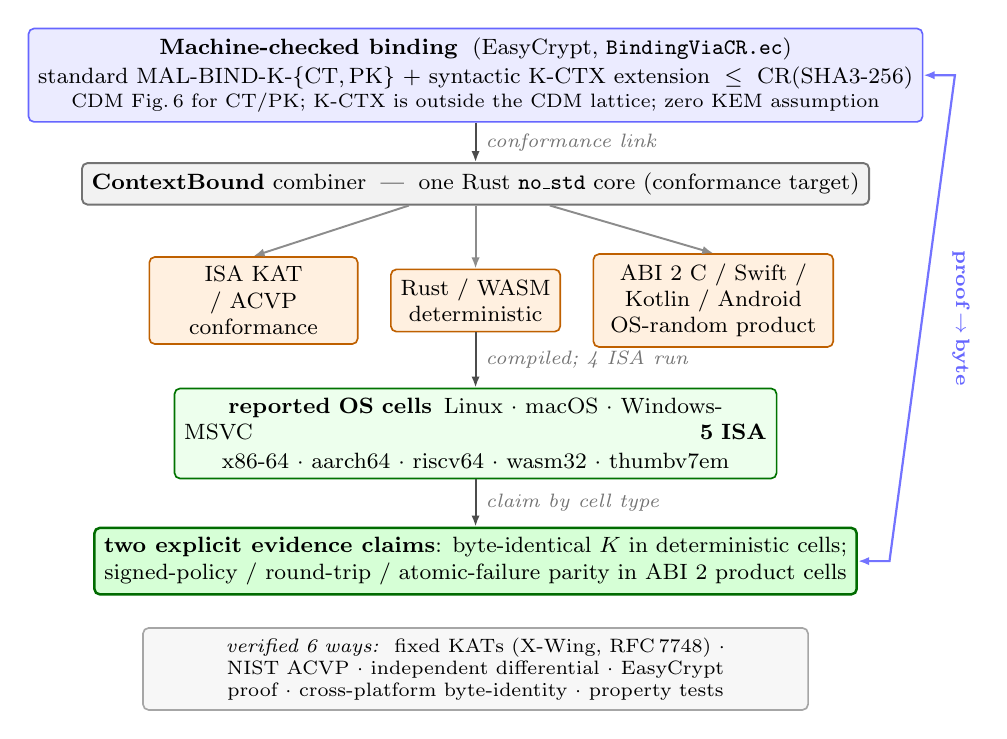
\begin{tikzpicture}[
  font=\footnotesize, >={Latex[length=4pt]},
  box/.style={draw, rounded corners=2pt, align=center, inner sep=3.5pt, line width=0.6pt},
  proof/.style={box, fill=blue!8, draw=blue!60},
  core/.style={box, fill=black!5, draw=black!55, line width=0.7pt},
  face/.style={box, fill=orange!12, draw=orange!75!black, minimum height=6mm, minimum width=11mm},
  sub/.style={box, fill=green!7, draw=green!45!black},
  result/.style={box, fill=green!16, draw=green!42!black, line width=0.9pt},
  lbl/.style={font=\scriptsize\itshape, text=black!55},
  flow/.style={->, line width=0.7pt, black!70},
]
% ---- proof (top) ----
\node[proof] (proof)
  {\textbf{Machine-checked binding} \;(EasyCrypt, \texttt{BindingViaCR.ec})\\[1pt]
   standard MAL-BIND-K-\{CT,\,PK\} $+$ syntactic K-CTX extension $\;\le\;$ CR(SHA3-256)\\[-1pt]
   {\scriptsize CDM Fig.\,6 for CT/PK; K-CTX is outside the CDM lattice; zero KEM assumption}};
% ---- single core ----
\node[core, below=5mm of proof] (core)
  {\textbf{ContextBound} combiner \;|\; one Rust \texttt{no\_std} core (conformance target)};
% ---- evidence planes (own row, centred under core) ----
\node[face, below=8mm of core] (f3) {Rust / WASM\\deterministic};
\node[face, left=4mm of f3, text width=24mm] (f2) {ISA KAT / ACVP\\conformance};
\node[face, right=4mm of f3, text width=28mm] (f4)
  {ABI~2 C / Swift / Kotlin / Android\\OS-random product};
% ---- substrate (below the faces row) ----
\node[sub, below=7mm of f3, text width=74mm] (substrate)
  {\textbf{reported OS cells}\, Linux $\cdot$ macOS $\cdot$ Windows-MSVC \hfill \textbf{5 ISA}\\[1pt]
   x86-64 $\cdot$ aarch64 $\cdot$ riscv64 $\cdot$ wasm32 $\cdot$ thumbv7em};
% ---- output: byte-identical K ----
\node[result, below=6mm of substrate] (k)
  {\textbf{two explicit evidence claims}: byte-identical $K$ in deterministic cells;\\
   signed-policy / round-trip / atomic-failure parity in ABI~2 product cells};
% ---- verification methods (footer) ----
\node[box, below=4mm of k, fill=black!3, draw=black!35, font=\scriptsize, text width=82mm] (ver)
  {\textit{verified 6 ways:}\, fixed KATs (X-Wing, RFC\,7748) $\cdot$ NIST ACVP $\cdot$ independent
   differential $\cdot$ EasyCrypt proof $\cdot$ cross-platform byte-identity $\cdot$ property tests};
% ---- arrows ----
\draw[flow] (proof) -- (core) node[midway, right, lbl] {conformance link};
\foreach \f in {f2,f3,f4} \draw[flow, black!45] (core) -- (\f.north);
\draw[flow] (f3) -- (substrate) node[midway, right, lbl] {compiled; 4 ISA run};
\draw[flow] (substrate) -- (k) node[midway, right, lbl] {claim by cell type};
% ---- proof-to-byte brace (right) ----
\coordinate (rt) at ($(proof.east)+(4mm,0)$);
\coordinate (rb) at ($(k.east)+(4mm,0)$);
\draw[{Latex[length=4pt]}-{Latex[length=4pt]}, line width=0.8pt, blue!55]
  (proof.east) -- (rt) -- (rb) -- (k.east);
\node[rotate=-90, font=\scriptsize\bfseries, text=blue!60, anchor=south]
  at ($(rt)!0.5!(rb)+(2.6mm,0)$) {proof\,$\to$\,byte};
\end{tikzpicture}
\end{document}
